% !TeX document-id = {3b8d65d3-a02c-4f16-abb9-6a325ca708dd}
% !TeX TXS-program:compile = txs:///latex/[--shell-escape]|txs:///dvips|txs:///ps2pdf
\documentclass[10pt]{article}
\usepackage[a4paper,bottom=3cm]{geometry}
\usepackage[spanish]{babel}
\usepackage[utf8]{inputenc}
\usepackage{fancyhdr} %header
\usepackage{amsmath}
\usepackage{amsfonts}
\usepackage{amssymb}
\usepackage{mdframed}
\usepackage{minted} % coloreado de codigo
\setminted{
	%bgcolor=gray!10,
	%	fontfamily=tt,
	linenos,
	breaklines,
	framesep = 3pt,
	frame=single
}
\usepackage{listings}
\usepackage{caption}
\usepackage{subcaption} % side by side figures
% pdf
\usepackage{hyperref}
% grafico
% grafo
\usepackage{float} % para forzar las imagenes
\usepackage[usenames,dvipsnames, pdf]{pstricks}
\usepackage{epsfig}
\usepackage{pst-grad} % For gradients
\usepackage{pst-plot} % For axes
\usepackage[space]{grffile} % For spaces in paths
\usepackage{etoolbox} % For spaces in paths
\makeatletter % For spaces in paths
\patchcmd\Gread@eps{\@inputcheck#1 }{\@inputcheck"#1"\relax}{}{}
% bug con minted
\makeatletter
\patchcmd{\minted@colorbg}{\noindent}{\medskip\noindent}{}{}
\apptocmd{\endminted@colorbg}{\par\medskip}{}{}
% minted: page breaks
%\surroundwithmdframed{minted}
\surroundwithmdframed[leftmargin=0pt,innerleftmargin=3pt,innertopmargin=3pt,
		rightmargin=0pt,innerrightmargin=3pt,innerbottommargin=3pt,topline=false,
		bottomline=false, leftline=false, rightline=false]{minted}
% \makeatother
%
\newcommand{\floor}[1]{\lfloor #1 \rfloor}

%
\author{Iñigo Biedma Ramos}
\title{Entrega Práctica Genéticos TSP}
\date{}
\renewcommand{\theenumi}{\alph{enumi}}
\pagestyle{fancy}
\fancyhf{}
\lhead{Entrega Práctica Genéticos TSP - Computación}
\rhead{Iñigo Biedma Ramos}
\begin{document}

\maketitle
\section{El problema}
Debemos resolver el problema del viajante (TSP), considerando las distancias entre las ciudades. Éstas van a ser simétricas, es decir que ir de la ciudad A a la ciudad B tendrá el mismo coste que ir de B a A. Resolveremos el problema para el caso genérico de N ciudades.
\subsection{Cromosomas}
Cada cromosoma representará una posible solución, indicando el orden en que visitaremos las ciudades. \textbf{Una solución va a consistir en un ciclo en el que sale de una ciudad y se vuelve a esa misma ciudad, visitando cada ciudad una vez.} Si numeramos las ciudades, y tenemos en cuenta que la ciudad de salida y de llegada es la misma y no hace falta escribirla dos veces, tendremos una permutación. Como definir una permutación es un poco complejo ($X_i = \bigl(\begin{smallmatrix}
1 & 2 & 3 & \cdots & N-1 & N \\2 & 3 & 4 & \cdots &  N  & 1\end{smallmatrix}\bigr)$, donde $X_i$ es una permutacion de los numeros de 1 a $N$) con notación matemática (esta notacion es de Cauchy), usaremos ejemplos.
$$(2,3,1,4,5) \text{ representa el ciclo } 2\rightarrow3\rightarrow 1\rightarrow4\rightarrow5\rightarrow2$$
\par
El objetivo es obtener el ciclo que menor distancia sume.Con N ciudades y para un ciclo determinado, existirán al menos N ciclos en los que la distancia es la misma.
% \usepackage[usenames,dvipsnames]{pstricks}
% \usepackage{epsfig}
% \usepackage{pst-grad} % For gradients
% \usepackage{pst-plot} % For axes
% \usepackage[space]{grffile} % For spaces in paths
% \usepackage{etoolbox} % For spaces in paths
% \makeatletter % For spaces in paths
% \patchcmd\Gread@eps{\@inputcheck#1 }{\@inputcheck"#1"\relax}{}{}
% \makeatother
% % User Packages:
% 
% 
\begin{figure}[H]
\begin{center}
\psscalebox{0.5 0.5} % Change this value to rescale the drawing.
{
\begin{pspicture}(0,-4.201433)(21.207233,4.201433)
\pscircle[linecolor=black, linewidth=0.04, dimen=outer](0.4001365,3.8012967){0.4001365}
\pscircle[linecolor=black, linewidth=0.04, dimen=outer](6.402184,3.8012967){0.4001365}
\pscircle[linecolor=black, linewidth=0.04, dimen=outer](6.402184,1.8006142){0.4001365}
\pscircle[linecolor=black, linewidth=0.04, dimen=outer](3.201092,0.60020477){0.4001365}
\pscircle[linecolor=black, linewidth=0.04, dimen=outer](2.0006826,2.2007508){0.4001365}
\psline[linecolor=black, linewidth=0.04](0.800273,3.8012967)(6.0020475,3.8012967)
\psline[linecolor=black, linewidth=0.04](6.402184,3.4011602)(6.402184,2.2007508)
\psline[linecolor=black, linewidth=0.04](6.0020475,1.8006142)(3.6012285,0.60020477)
\pscircle[linecolor=black, linewidth=0.04, dimen=outer](0.4001365,1.4004778){0.4001365}
\psline[linecolor=black, linewidth=0.04](2.8009555,0.60020477)(2.0006826,1.8006142)
\psline[linecolor=black, linewidth=0.04](1.600546,2.2007508)(0.800273,1.4004778)
\psline[linecolor=black, linewidth=0.04](0.4001365,1.8006142)(0.4001365,3.4011602)
\pscircle[linecolor=black, linewidth=0.04, dimen=outer](0.4001365,3.8012967){0.4001365}
\psdots[linecolor=black, dotsize=0.36755615](0.40487346,3.7965598)
\pscircle[linecolor=black, linewidth=0.04, dimen=outer](7.6025934,3.8012967){0.4001365}
\pscircle[linecolor=black, linewidth=0.04, dimen=outer](13.604641,3.8012967){0.4001365}
\pscircle[linecolor=black, linewidth=0.04, dimen=outer](13.604641,1.8006142){0.4001365}
\pscircle[linecolor=black, linewidth=0.04, dimen=outer](10.403549,0.60020477){0.4001365}
\pscircle[linecolor=black, linewidth=0.04, dimen=outer](9.203139,2.2007508){0.4001365}
\psline[linecolor=black, linewidth=0.04](8.00273,3.8012967)(13.204504,3.8012967)
\psline[linecolor=black, linewidth=0.04](13.604641,3.4011602)(13.604641,2.2007508)
\psline[linecolor=black, linewidth=0.04](13.204504,1.8006142)(10.803685,0.60020477)
\pscircle[linecolor=black, linewidth=0.04, dimen=outer](7.6025934,1.4004778){0.4001365}
\psline[linecolor=black, linewidth=0.04](10.003412,0.60020477)(9.203139,1.8006142)
\psline[linecolor=black, linewidth=0.04](8.803003,2.2007508)(8.00273,1.4004778)
\psline[linecolor=black, linewidth=0.04](7.6025934,1.8006142)(7.6025934,3.4011602)
\pscircle[linecolor=black, linewidth=0.04, dimen=outer](7.6025934,3.8012967){0.4001365}
\psdots[linecolor=black, dotsize=0.4001365](13.604874,3.7965598)
\pscircle[linecolor=black, linewidth=0.04, dimen=outer](14.805051,3.8012967){0.4001365}
\pscircle[linecolor=black, linewidth=0.04, dimen=outer](20.807098,3.8012967){0.4001365}
\pscircle[linecolor=black, linewidth=0.04, dimen=outer](20.807098,1.8006142){0.4001365}
\pscircle[linecolor=black, linewidth=0.04, dimen=outer](17.606007,0.60020477){0.4001365}
\pscircle[linecolor=black, linewidth=0.04, dimen=outer](16.405596,2.2007508){0.4001365}
\psline[linecolor=black, linewidth=0.04](15.205187,3.8012967)(20.406961,3.8012967)
\psline[linecolor=black, linewidth=0.04](20.807098,3.4011602)(20.807098,2.2007508)
\psline[linecolor=black, linewidth=0.04](20.406961,1.8006142)(18.006142,0.60020477)
\pscircle[linecolor=black, linewidth=0.04, dimen=outer](14.805051,1.4004778){0.4001365}
\psline[linecolor=black, linewidth=0.04](17.20587,0.60020477)(16.405596,1.8006142)
\psline[linecolor=black, linewidth=0.04](16.00546,2.2007508)(15.205187,1.4004778)
\psline[linecolor=black, linewidth=0.04](14.805051,1.8006142)(14.805051,3.4011602)
\pscircle[linecolor=black, linewidth=0.04, dimen=outer](14.805051,3.8012967){0.4001365}
\psdots[linecolor=black, dotsize=0.4001365](20.804874,1.7965598)
\pscircle[linecolor=black, linewidth=0.04, dimen=outer](0.4001365,-0.60020477){0.4001365}
\pscircle[linecolor=black, linewidth=0.04, dimen=outer](6.402184,-0.60020477){0.4001365}
\pscircle[linecolor=black, linewidth=0.04, dimen=outer](6.402184,-2.6008873){0.4001365}
\pscircle[linecolor=black, linewidth=0.04, dimen=outer](3.201092,-3.8012967){0.4001365}
\pscircle[linecolor=black, linewidth=0.04, dimen=outer](2.0006826,-2.2007508){0.4001365}
\psline[linecolor=black, linewidth=0.04](0.800273,-0.60020477)(6.0020475,-0.60020477)
\psline[linecolor=black, linewidth=0.04](6.402184,-1.0003413)(6.402184,-2.2007508)
\psline[linecolor=black, linewidth=0.04](6.0020475,-2.6008873)(3.6012285,-3.8012967)
\pscircle[linecolor=black, linewidth=0.04, dimen=outer](0.4001365,-3.0010238){0.4001365}
\psline[linecolor=black, linewidth=0.04](2.8009555,-3.8012967)(2.0006826,-2.6008873)
\psline[linecolor=black, linewidth=0.04](1.600546,-2.2007508)(0.800273,-3.0010238)
\psline[linecolor=black, linewidth=0.04](0.4001365,-2.6008873)(0.4001365,-1.0003413)
\pscircle[linecolor=black, linewidth=0.04, dimen=outer](0.4001365,-0.60020477){0.4001365}
\psdots[linecolor=black, dotsize=0.4001365](0.40487346,-3.0034401)
\pscircle[linecolor=black, linewidth=0.04, dimen=outer](7.6025934,-0.60020477){0.4001365}
\pscircle[linecolor=black, linewidth=0.04, dimen=outer](13.604641,-0.60020477){0.4001365}
\pscircle[linecolor=black, linewidth=0.04, dimen=outer](13.604641,-2.6008873){0.4001365}
\pscircle[linecolor=black, linewidth=0.04, dimen=outer](10.403549,-3.8012967){0.4001365}
\pscircle[linecolor=black, linewidth=0.04, dimen=outer](9.203139,-2.2007508){0.4001365}
\psline[linecolor=black, linewidth=0.04](8.00273,-0.60020477)(13.204504,-0.60020477)
\psline[linecolor=black, linewidth=0.04](13.604641,-1.0003413)(13.604641,-2.2007508)
\psline[linecolor=black, linewidth=0.04](13.204504,-2.6008873)(10.803685,-3.8012967)
\pscircle[linecolor=black, linewidth=0.04, dimen=outer](7.6025934,-3.0010238){0.4001365}
\psline[linecolor=black, linewidth=0.04](10.003412,-3.8012967)(9.203139,-2.6008873)
\psline[linecolor=black, linewidth=0.04](8.803003,-2.2007508)(8.00273,-3.0010238)
\psline[linecolor=black, linewidth=0.04](7.6025934,-2.6008873)(7.6025934,-1.0003413)
\pscircle[linecolor=black, linewidth=0.04, dimen=outer](7.6025934,-0.60020477){0.4001365}
\psdots[linecolor=black, dotsize=0.4001365](9.204873,-2.2034402)
\pscircle[linecolor=black, linewidth=0.04, dimen=outer](14.805051,-0.60020477){0.4001365}
\pscircle[linecolor=black, linewidth=0.04, dimen=outer](20.807098,-0.60020477){0.4001365}
\pscircle[linecolor=black, linewidth=0.04, dimen=outer](20.807098,-2.6008873){0.4001365}
\pscircle[linecolor=black, linewidth=0.04, dimen=outer](17.606007,-3.8012967){0.4001365}
\pscircle[linecolor=black, linewidth=0.04, dimen=outer](16.405596,-2.2007508){0.4001365}
\psline[linecolor=black, linewidth=0.04](15.205187,-0.60020477)(20.406961,-0.60020477)
\psline[linecolor=black, linewidth=0.04](20.807098,-1.0003413)(20.807098,-2.2007508)
\psline[linecolor=black, linewidth=0.04](20.406961,-2.6008873)(18.006142,-3.8012967)
\pscircle[linecolor=black, linewidth=0.04, dimen=outer](14.805051,-3.0010238){0.4001365}
\psline[linecolor=black, linewidth=0.04](17.20587,-3.8012967)(16.405596,-2.6008873)
\psline[linecolor=black, linewidth=0.04](16.00546,-2.2007508)(15.205187,-3.0010238)
\psline[linecolor=black, linewidth=0.04](14.805051,-2.6008873)(14.805051,-1.0003413)
\pscircle[linecolor=black, linewidth=0.04, dimen=outer](14.805051,-0.60020477){0.4001365}
\psdots[linecolor=black, dotsize=0.4001365](17.604874,-3.8034403)
\end{pspicture}
}
\end{center}
\caption{6 ciclos iguales con diferentes ciudades de inicio}
\end{figure}


Por esta razón, podemos fijar una de las ciudades como ciudad de origen y reduciremos la complejidad de nuestro algoritmo. No includiremos la ciudad N en nuestros cromosomas, aunque si tendremos que considerarla al calcular las distancias. Por tanto el vector $[2\ 3\ 1\ 4]$ representa el ciclo $5\rightarrow2\rightarrow 3\rightarrow1\rightarrow4\rightarrow5$
\par
En el guión se nos indica que en cada ejecución del programa generaremos una matriz con las distancias emtre las ciudades. Esta matriz es simétrica
\[
MatDis=
\begin{pmatrix}
0 & d_{1,2} & d_{1,3} & d_{1,4} & d_{1,5} \\
d_{1,2} & 0 & d_{2,3} & d_{2,4} & d_{2,5} \\
d_{1,3} & d_{2,3} & 0 & d_{3,4} & d_{3,5} \\
d_{1,4} & d_{2,4} & d_{3,4} & 0 & d_{4,5} \\
d_{1,5} & d_{2,5} & d_{3,5} & d_{4,5} & 0 \\
\end{pmatrix}
\text{tq }d_{j,i}=d_{i,j}\text{ es la distancia de }i\text{ a }j
\]
El algoritmo lo vamos a codificar en matlab, y para representar las permutaciones utilizaremos vectores. Para el vector $[2\ 3\ 1\ 4]$ tendremos que sumar  $$distancia([2\ 3\ 1\ 4])=d_{5,2}+d_{2,3}+d_{3,1}+d_{1,4}+d_{4,5}$$
En matlab es difícil tomar varios elementos a la vez de una matriz de varias dimensiones y se debe usar $sub2ind$. En cada iteración del algoritmo tendríamos que usar muchas veces esta función y eso ralentizarña el código. Lo vamos a evitar mapeando la matriz de distancias a un vector, de forma que tengamos una forma mucho más rápida de obtener las distancias que necesitamos.\par
Este vector $VDis$ tendrá $d_{i,j}$ en la posición $\lambda i+j$ donde $lambda = 10^{\floor{\log_{10}N}}$. Es decir para el caso de $N < 10$ tendremos $d_{5,8}$ en $VDis[58]$, para $9 < N < 100$ en $VDis[508]$ y $d_{23,12}$ en $VDis[2312]$. Habrá muchas posiciones que estén vacías pero el coste en memoria es ínfimo en comparación el computacional. Podemos calcular la distancia de un cromosoma en unas pocas operaciones:
\begin{minted}{matlab}
distancias = sum(VDis([ones(tamPob,1, 'like', tamPob)*N Pob]*LN+[Pob ones(tamPob,1, 'like', tamPob)*N]),2);
\end{minted}
El codigo anterior toma la matriz en la cual en cada fila tenemos un cromosoma y obtiene las posiciones que sumaremos, para luego sumar. Con N=4 y un vector:
$$[1\ 2\ 3] \rightarrow [\textbf{4}\ 1\ 2\ 3]*10 + [1\ 2\ 3\ \textbf{4}] \rightarrow [41\ 12\ 23\ 34]$$
Con $N=7$ y en matlab:
\begin{Verbatim}
>> Pob
4      1      5      2      6      3
1      5      6      2      3      4
5      1      4      3      2      6
1      4      5      3      2      6
4      2      5      1      3      6
>> [ones(tamPob,1, 'like', tamPob)*N Pob]*LN+[Pob ones(tamPob,1, 'like', tamPob)*N]
74     41     15     52     26     63     37
71     15     56     62     23     34     47
75     51     14     43     32     26     67
71     14     45     53     32     26     67
74     42     25     51     13     36     67

\end{Verbatim}
\pagebreak
\subsection{Función de fitness}
Las distancias es una buena medida de lo bueno o malo que es un cromosoma. Por definición la función de fitness debe tener un valor mayor cuanto mejor es un cromosoma, inversamente proporcional a la distancia. Nuestra primera aproximación fue $distancia^{-1}$.
\begin{figure}[h]
		\begin{subfigure}[t]{0.50\textwidth}
			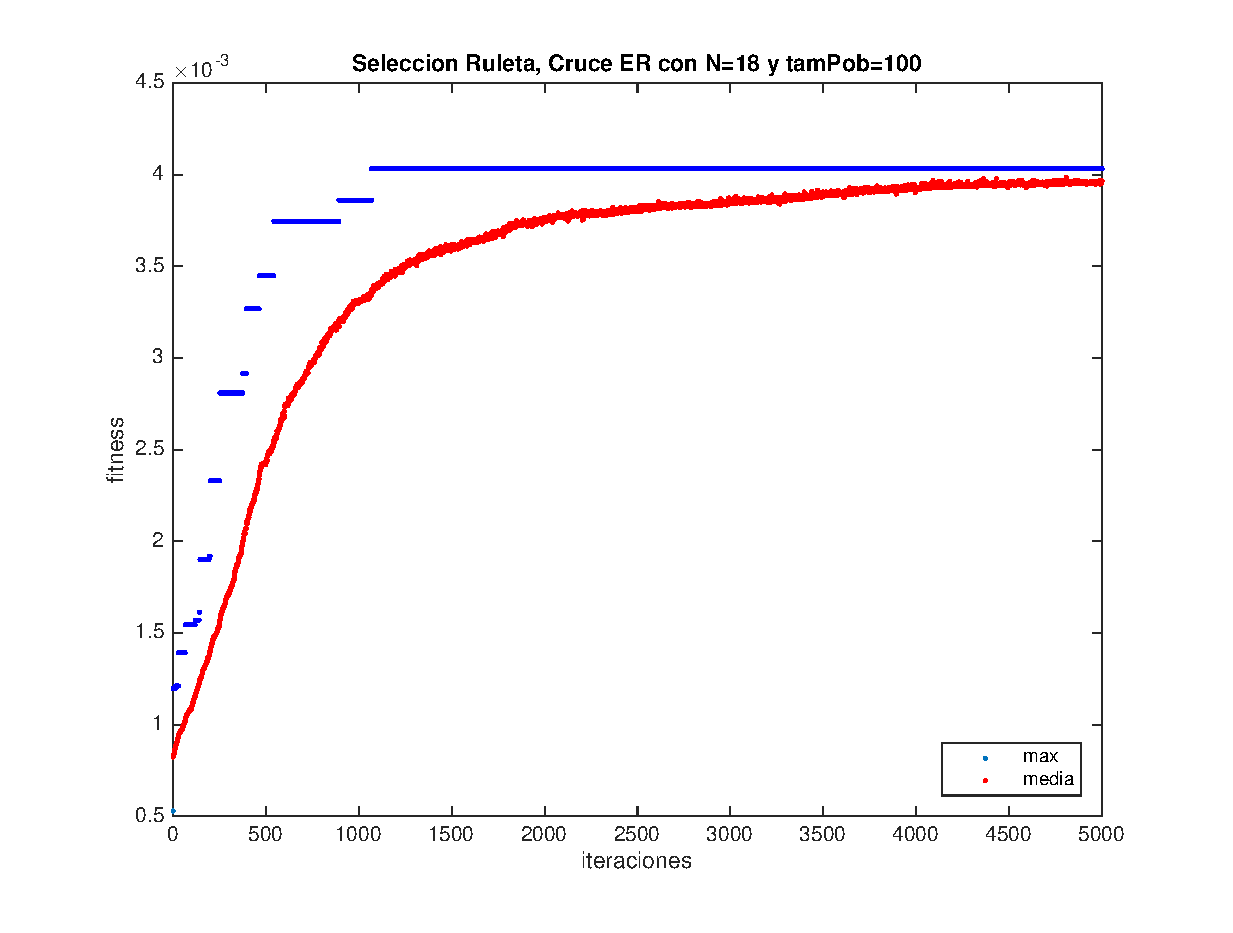
\includegraphics[width=\linewidth]{N18S1ERP100}
		\end{subfigure}
		\begin{subfigure}[t]{0.50\textwidth}
			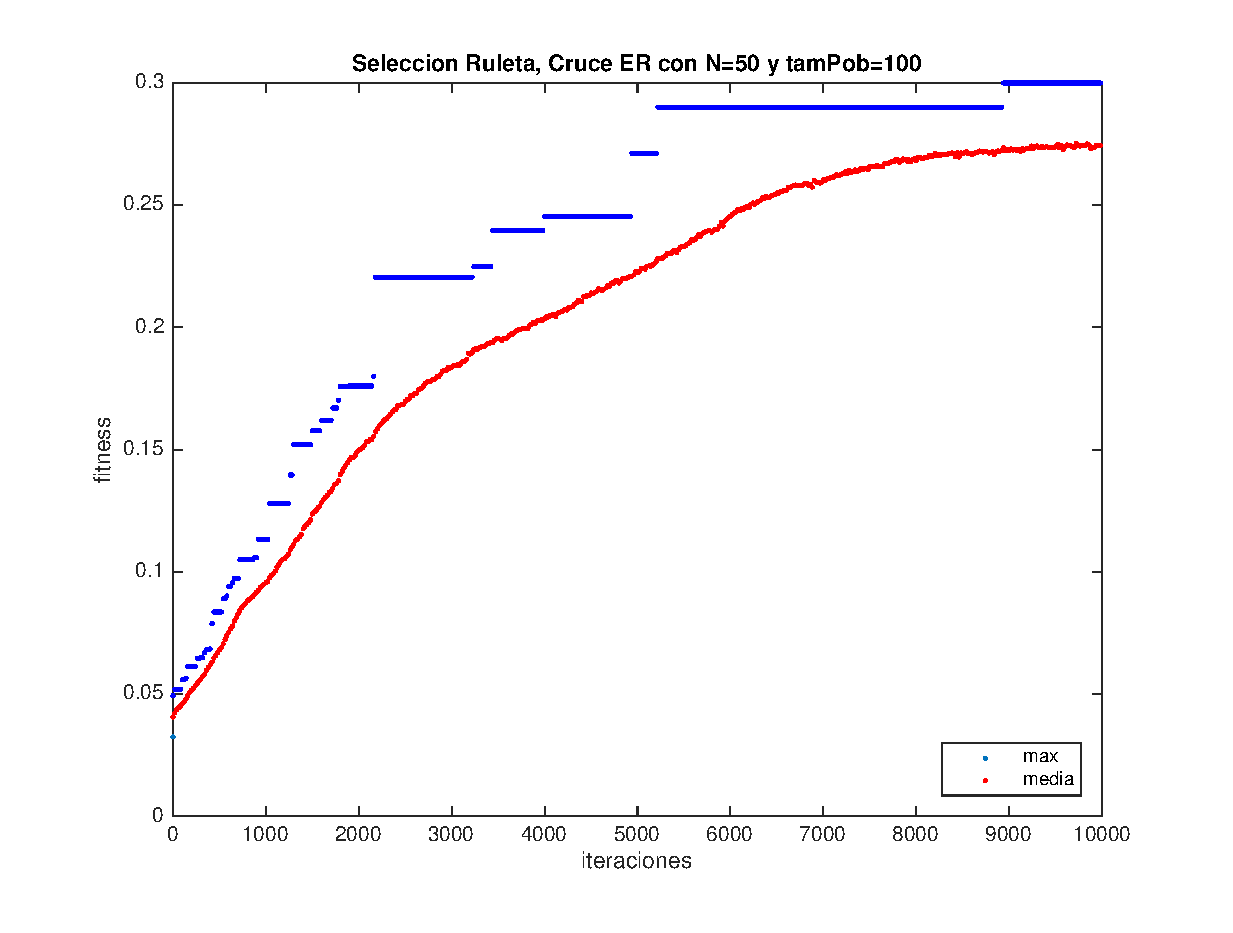
\includegraphics[width=\linewidth]{N50S1ERP100_17}
		\end{subfigure}
	\caption{con $distancia^{-1}$ quedan valores de fitness muy pequeños. Usando $\frac{maxDist}{distancia}$ obtenemos resultados más cómodos. La figura de la derecha corresponde a este caso.}
\end{figure}
Para casos sencillos, y para comparar las variaciones del algoritmo con más facilidad, calcularemos antes el mejor resultado y utilizaremos $\frac{mejorDistancia}{distancia}$. En tal caso cuando el fitness llegue a 1 tendremos el mejor resultado.
\subsection{Cruzamiento}
Para el cruzamiento he programado dos métodos: cruzamiento basado en orden (OX) y cruzamiento de aristas (ER). He elegido estos dos después de leer un par de documentos en los que ponen a prueba varios métodos \cite{jess} y concluyen que son los mejores \cite{larra}. Además, el de orden es mucho más rápido.\\
Para N=15 y 10000 iteraciones, OX demora 0.452s y ER 3.339s (Midiendo el tiempo consumido por la función de cruce).
\begin{figure}[H]
	\begin{subfigure}[H]{0.50\textwidth}
		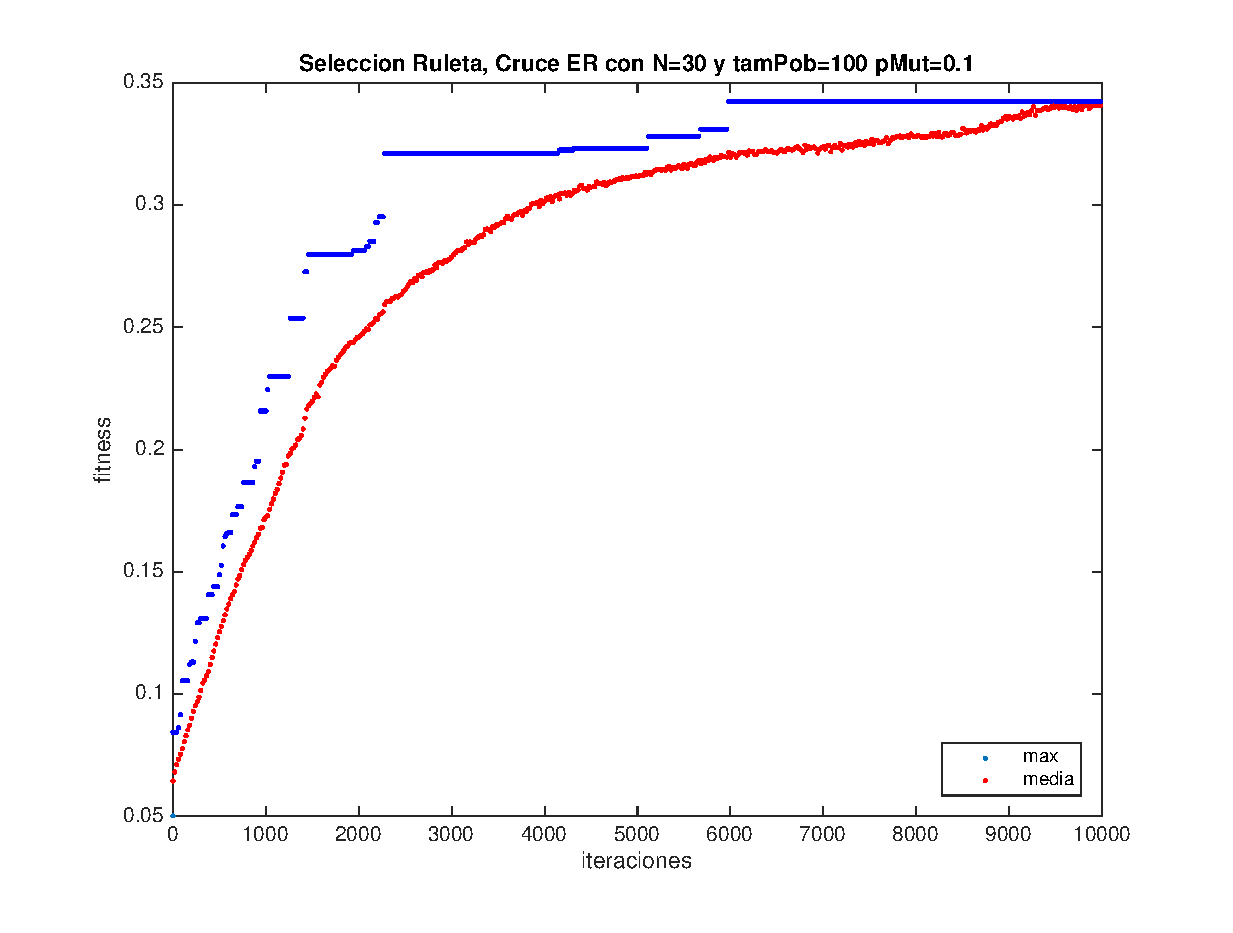
\includegraphics[width=\linewidth]{N30S1ERP100_24}
	\end{subfigure}
	\begin{subfigure}[H]{0.50\textwidth}
		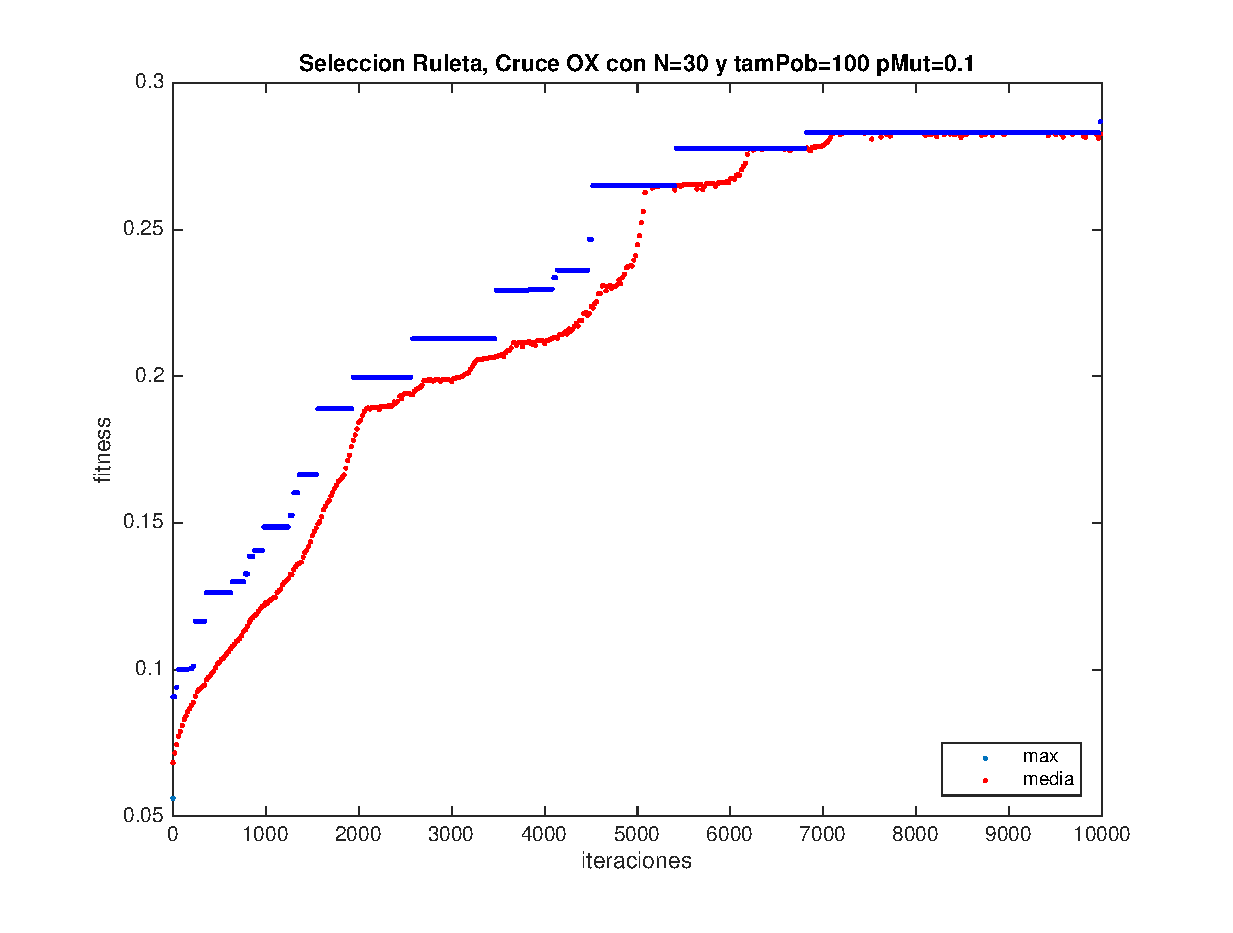
\includegraphics[width=\linewidth]{N30S1OXP100_25}
	\end{subfigure}
	\caption{El cruce OX suele converger más deprisa, pero a veces se estanca en mínimos locales}
\end{figure}
\subsection{Seleccion}
Hemos utilizado los metodos de la ruleta y del torneo. El del torneo converge más rápidamente, pero es muy elitista. Al tomar el de mejor fitness del subconjunto elegido al azar es imposible que los k-1 cromosomas peores sean elegidos como padres.
\begin{figure}[H]
	\begin{subfigure}[H]{0.50\textwidth}
		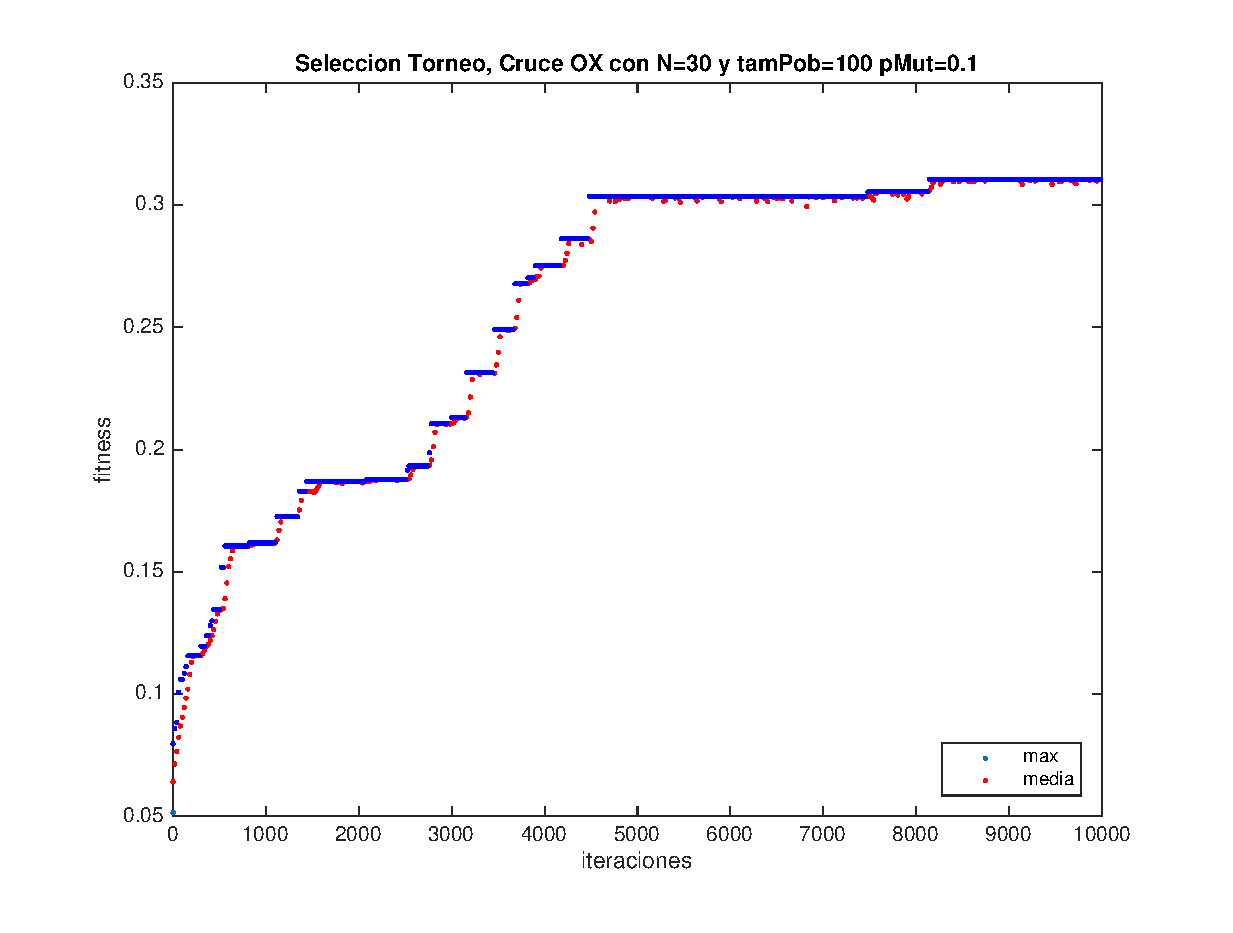
\includegraphics[width=\linewidth]{N30S2OXP100_29}
	\end{subfigure}%
	\begin{subfigure}[H]{0.50\textwidth}
		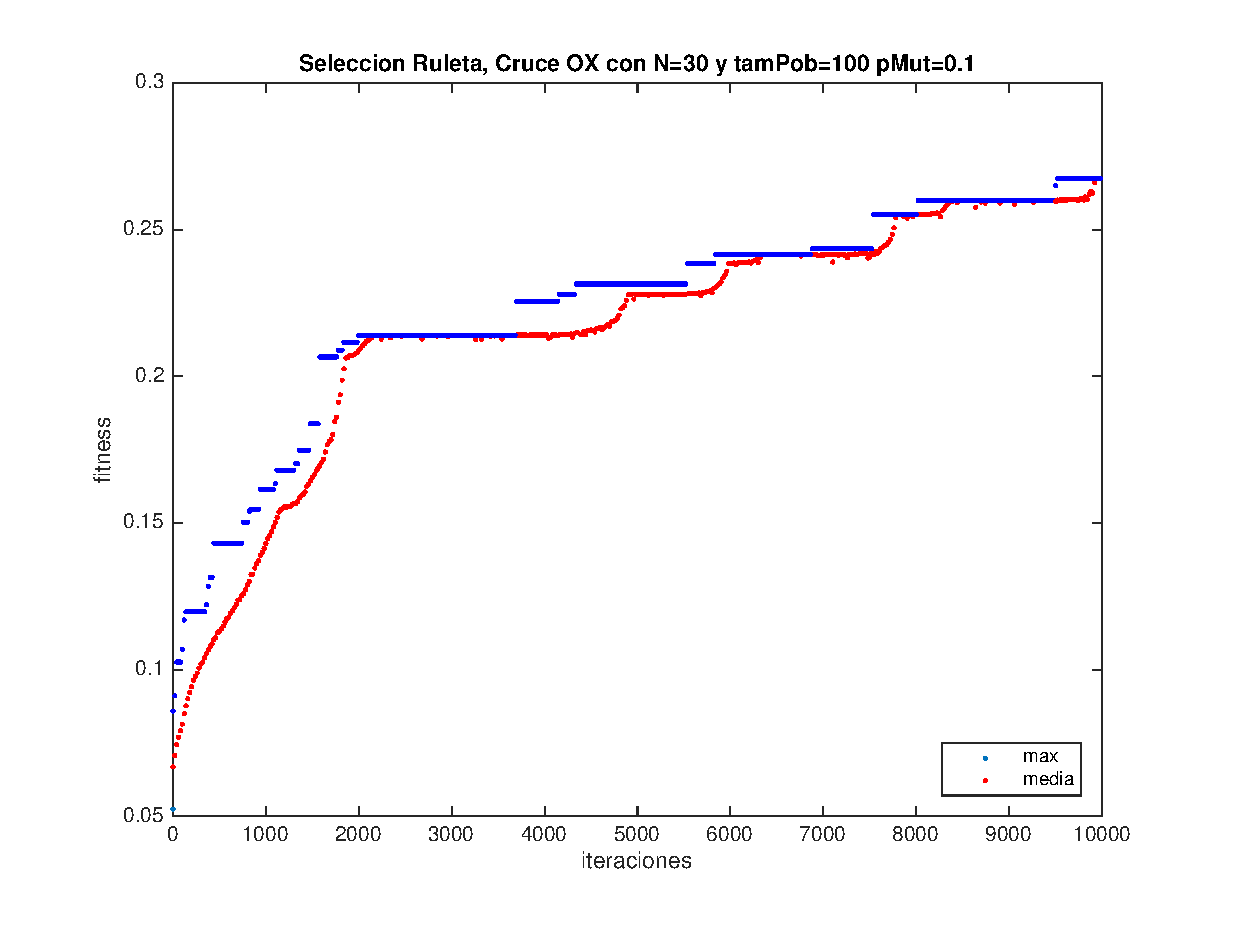
\includegraphics[width=\linewidth]{N30S1OXP100_27}
	\end{subfigure}
	\begin{subfigure}[H]{0.50\textwidth}
		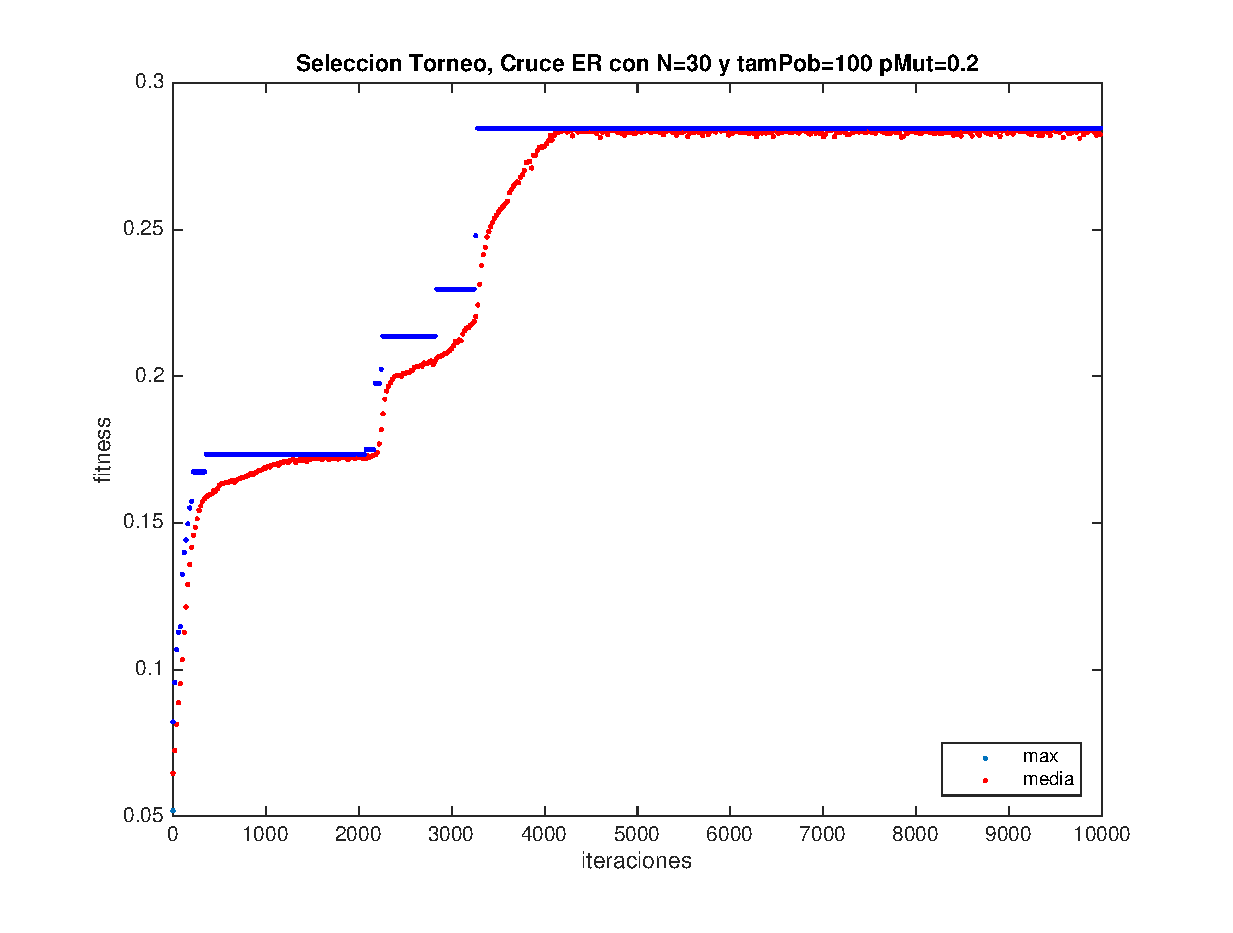
\includegraphics[width=\linewidth]{N30S2ERP100_34}
	\end{subfigure}%
	\begin{subfigure}[H]{0.50\textwidth}
		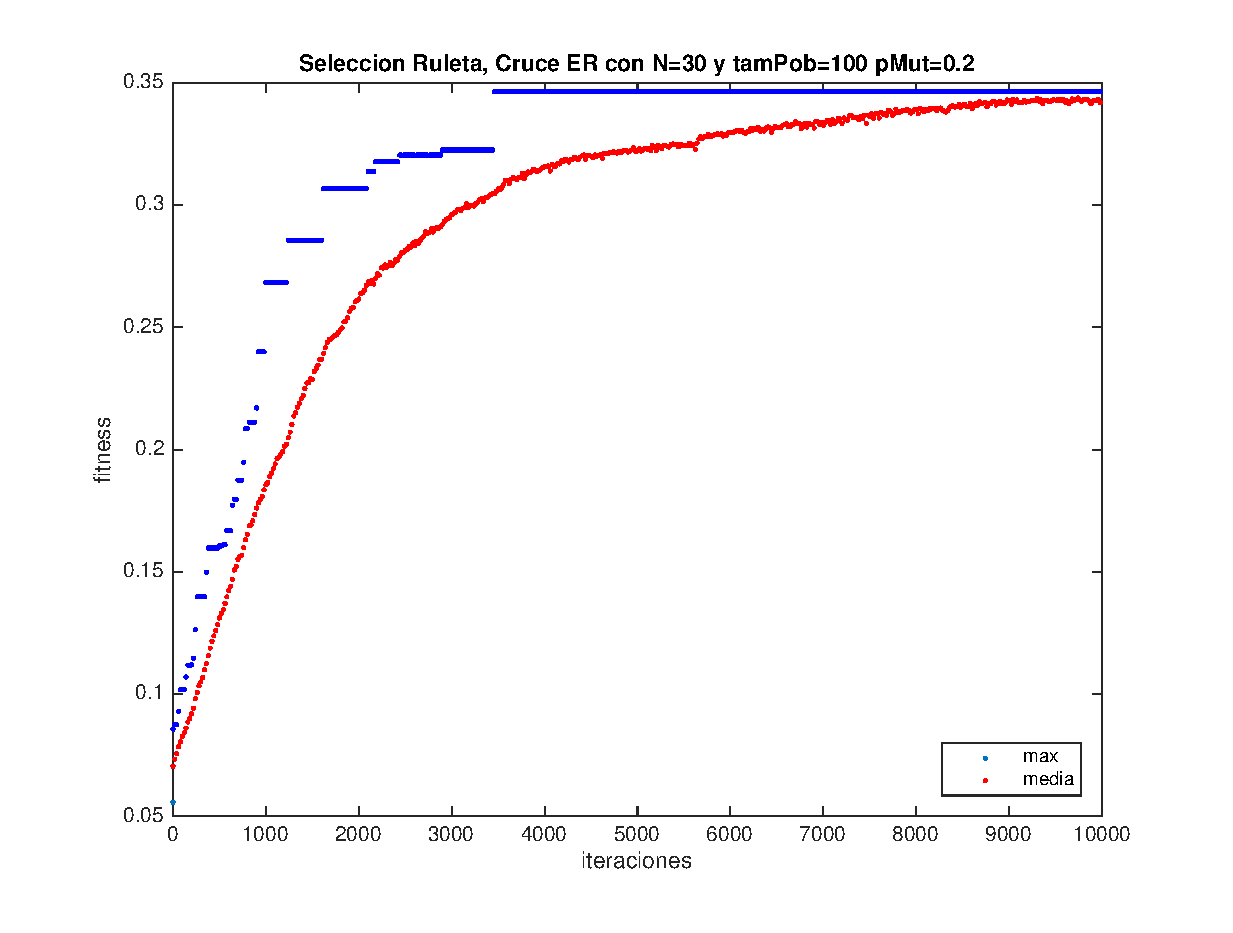
\includegraphics[width=\linewidth]{N30S1ERP100_33}
	\end{subfigure}%
	\caption{Haciendo seleccion por torneo enseguida la población cambia para parecerse al mejor individuo}
\end{figure}
\par
\subsection{Mutación}
Hemos codificado los 3 métodos de mutación para permutaciones vistos en clase: Inserción, sacudida e inversión\\
Aparentemente no se aprecia una diferencia relevante entre la probabilidad de mntación y el fitness obtenido en la última iteración, pero si la hay respecto a la convergencia. Si la población es grande una mala mutación no afectará mucho a la población entera, pero si la población es pequeña podría empeorar el resultado.
\subsection{Numero de ciudades}
El numero de ciudades, N, es el parámetro más importante. Si se intenta calcular la solución por fuerza bruta tendremos $N!$ posibles permutaciones, siendo imposible calcularlo a partir de cierto N. 
\section{Analizando los parámetros}
Para analizar y comparar diferentes métodos, es necesario prefijar los parámetros independientes a dichos métodos. Cada vez que se ejecuta el código calculamos una matriz de distancias, pero para comparar parámetros nos interesa considerar el mismo problema todo el tiempo. \\ 
La variable que nos va a indicar lo bien o mal que está resolviendo el problema el algoritmo va a ser el fitness. Este va depender de la distancia, y como cada vez que ejcutamos tenemos una matriz de distancias diferentes, no podemos comparar dos valores de fitness entre sí.\\
Ésto lo solucionamos comparando nuestro algoritmo con la solución óptima. Para valores bajos de N podemos calcular la solución por fuerza bruta en unos pocos segundos. Está codificado de una manera muy poco óptima pero nos vale. \\
Para valores mayores de N, podemos tomar ejemplos cuya solución óptima es conocida. De TSPlib \cite{TSPlib} hemos tomado el problema "bay29", para comparar nuestros parámetros en un caso de $N=29$.
\begin{mdframed}
	Muchas de las pruebas que he realizado del algoritmo las he registrado en un archivo del que muestro aquí algunas líneas. Su estructura es la siguiente:
	\begin{Verbatim}[fontsize=\small]
	N=<N> <maxiteraciones>i (<iteraciones utiles>) P <tamPob>
	pM<metodoMutacion> <probMutacion> <metodoSeleccion> <metodoCruce> 
	:: fit <fitness maximo> <distancia minima>/<distancia referencia>
	:: t:<tiempo_total>s
	\end{Verbatim}
	Las iteraciones útiles es el numero de iteraciones realizadas hasta alcanzar el máximo fitness. Llamada $mejorDistancia$ anteriormente.
\end{mdframed}
\paragraph{N}N determina la complejidad del problema.  En el genético, para un N mayor necesitaremos más iteraciones hasta dar con una mejor solución.
Resultados:
\begin{verbatim}
5e3 iter Cruce aleatorio:
N= 10    5000i (     410) P 50 pM3 0.81  Ruleta ER :: fit 1.00 BD  269/ 269 :: t:1.396s
N= 15    5000i (    1023) P 50 pM1 0.15  Torneo OX :: fit 0.36 BD  414/ 150 :: t:0.629s
N= 20    5000i (    3331) P 50 pM2 0.84  Ruleta ER :: fit 0.40 BD  371/ 150 :: t:2.356s
N= 25    5000i (    1258) P 50 pM2 0.06  Ruleta ER :: fit 0.35 BD  431/ 150 :: t:2.498s
N= 30    5000i (    3850) P 50 pM2 0.66  Torneo ER :: fit 0.17 BD  871/ 150 :: t:2.628s
N= 35    5000i (    4931) P 50 pM2 0.85  Ruleta ER :: fit 0.27 BD  559/ 150 :: t:4.312s
N= 40    5000i (    4500) P 50 pM3 0.24  Torneo ER :: fit 0.13 BD 1116/ 150 :: t:3.157s
N= 45    5000i (    4085) P 50 pM2 0.09  Torneo OX :: fit 0.09 BD 1660/ 150 :: t:0.469s
N= 50    5000i (    4517) P 50 pM1 0.32  Ruleta ER :: fit 0.20 BD  735/ 150 :: t:6.303s
N= 55    5000i (    4801) P 50 pM2 0.03  Torneo OX :: fit 0.07 BD 2090/ 150 :: t:0.588s
N= 60    5000i (    4678) P 50 pM1 0.56  Torneo OX :: fit 0.11 BD 1409/ 150 :: t:1.151s
N= 65    5000i (    2683) P 50 pM3 0.09  Torneo ER :: fit 0.06 BD 2419/ 150 :: t:5.223s
N= 70    5000i (    4781) P 50 pM3 0.00  Torneo OX :: fit 0.04 BD 3406/ 150 :: t:0.447s
N= 75    5000i (    3948) P 50 pM3 0.92  Torneo ER :: fit 0.12 BD 1280/ 150 :: t:6.315s
N= 80    5000i (    4901) P 50 pM2 0.85  Torneo ER :: fit 0.06 BD 2359/ 150 :: t:6.503s
N= 85    5000i (    4567) P 50 pM2 0.53  Torneo OX :: fit 0.06 BD 2677/ 150 :: t:0.521s
N= 90    5000i (    4355) P 50 pM2 0.17  Torneo ER :: fit 0.04 BD 3355/ 150 :: t:7.179s
N= 95    5000i (    4981) P 50 pM1 0.25  Ruleta OX :: fit 0.07 BD 2077/ 150 :: t:0.671s
N=100    5000i (    4939) P 50 pM2 0.75  Ruleta OX :: fit 0.10 BD 1474/ 150 :: t:0.562s
N=105    5000i (    3803) P 50 pM2 0.18  Ruleta OX :: fit 0.02 BD 6554/ 150 :: t:0.536s
N=110    5000i (    4957) P 50 pM1 0.35  Ruleta OX :: fit 0.04 BD 3458/ 150 :: t:0.797s
N=115    5000i (    4675) P 50 pM2 0.99  Ruleta ER :: fit 0.03 BD 4314/ 150 :: t:16.562s
N=120    5000i (    4676) P 50 pM2 0.64  Torneo ER :: fit 0.02 BD 9773/ 150 :: t:9.572s
N=125    5000i (    2272) P 50 pM3 0.14  Torneo ER :: fit 0.02 BD 9759/ 150 :: t:9.777s
N=130    5000i (    4944) P 50 pM1 0.91  Ruleta ER :: fit 0.02 BD 8338/ 150 :: t:18.290s
N=135    5000i (    4874) P 50 pM2 0.18  Ruleta ER :: fit 0.02 BD 7102/ 150 :: t:14.631s
N=140    5000i (    4561) P 50 pM2 0.23  Torneo ER :: fit 0.03 BD 4840/ 150 :: t:11.251s
N=145    5000i (    4973) P 50 pM1 0.09  Torneo OX :: fit 0.05 BD 3317/ 150 :: t:0.670s
N=150    5000i (    2664) P 50 pM3 0.64  Ruleta ER :: fit 0.01 BD 10814/ 150 :: t:18.402s

50e3 iter Cruce aleatorio:
N=  5   50000i () P 50 pM3 0.26  Ruleta ER :: fit 1.00 BD  348/ 348 :: t:5.312s
N= 10   50000i (     202) P 50 pM3 0.42  Ruleta ER :: fit 1.00 BD  301/ 301 :: t:8.864s
N= 15   50000i (     253) P 50 pM1 0.23  Torneo OX :: fit 0.32 BD  465/ 150 :: t:4.729s
N= 20   50000i (    3171) P 50 pM2 0.88  Ruleta OX :: fit 0.36 BD  417/ 150 :: t:3.671s
N= 25   50000i (    3155) P 50 pM2 0.60  Torneo OX :: fit 0.30 BD  503/ 150 :: t:3.699s
N= 30   50000i (   28334) P 50 pM2 0.04  Ruleta ER :: fit 0.24 BD  621/ 150 :: t:22.798s
N= 35   50000i (   10380) P 50 pM3 0.57  Ruleta OX :: fit 0.37 BD  405/ 150 :: t:3.454s
N= 40   50000i (    3216) P 50 pM1 0.53  Ruleta OX :: fit 0.20 BD  745/ 150 :: t:7.167s
N= 45   50000i (   36187) P 50 pM2 0.61  Torneo ER :: fit 0.12 BD 1262/ 150 :: t:33.636s
N= 50   50000i (   38840) P 50 pM2 0.94  Torneo OX :: fit 0.12 BD 1238/ 150 :: t:4.289s
N= 55   50000i (   37340) P 50 pM1 0.61  Ruleta ER :: fit 0.28 BD  545/ 150 :: t:47.521s
N= 60   50000i (    9849) P 50 pM3 0.61  Torneo OX :: fit 0.33 BD  456/ 150 :: t:3.919s
N= 65   50000i (   48286) P 50 pM3 0.71  Ruleta ER :: fit 0.25 BD  593/ 150 :: t:54.157s
N= 70   50000i (   48509) P 50 pM3 0.84  Torneo ER :: fit 0.16 BD  912/ 150 :: t:53.762s
N= 75   50000i (   41014) P 50 pM3 0.17  Torneo OX :: fit 0.25 BD  612/ 150 :: t:3.811s
N= 80   50000i (   49910) P 50 pM1 0.30  Ruleta OX :: fit 0.12 BD 1304/ 150 :: t:5.948s
N= 85   50000i (   33672) P 50 pM1 0.19  Ruleta OX :: fit 0.10 BD 1549/ 150 :: t:5.208s
N= 90   50000i (   30024) P 50 pM2 0.73  Torneo ER :: fit 0.05 BD 2971/ 150 :: t:68.469s
N= 95   50000i (   47828) P 50 pM3 0.09  Torneo OX :: fit 0.20 BD  732/ 150 :: t:3.899s
N=100   50000i (   41466) P 50 pM1 0.29  Torneo OX :: fit 0.19 BD  808/ 150 :: t:6.355s
N=105   50000i (   47126) P 50 pM1 0.37  Ruleta ER :: fit 0.06 BD 2690/ 150 :: t:89.962s
N=110   50000i (   43428) P 50 pM2 0.59  Ruleta ER :: fit 0.02 BD 6530/ 150 :: t:96.370s
N=115   50000i (   49613) P 50 pM2 0.47  Ruleta ER :: fit 0.05 BD 2761/ 150 :: t:98.154s
N=120   50000i (   49842) P 50 pM1 0.28  Ruleta ER :: fit 0.02 BD 7485/ 150 :: t:99.681s
N=125   50000i (   49442) P 50 pM1 0.11  Ruleta ER :: fit 0.02 BD 7265/ 150 :: t:100.680s

50e3 iter Cruce OX:
N=  5   50000i () P 50 pM3 0.86  Ruleta OX :: fit 1.00 BD  381/ 381 :: t:3.201s
N= 10   50000i (   17407) P 50 pM3 0.64  Torneo OX :: fit 1.00 BD  208/ 208 :: t:3.422s
N= 15   50000i (    8329) P 50 pM2 0.57  Ruleta OX :: fit 0.50 BD  300/ 150 :: t:3.346s
N= 20   50000i (    1577) P 50 pM1 0.23  Torneo OX :: fit 0.24 BD  613/ 150 :: t:4.888s
N= 25   50000i (   39142) P 50 pM2 0.88  Torneo OX :: fit 0.36 BD  414/ 150 :: t:3.904s
N= 30   50000i (   47361) P 50 pM2 0.40  Torneo OX :: fit 0.22 BD  667/ 150 :: t:3.563s
N= 35   50000i (    8993) P 50 pM1 0.96  Ruleta OX :: fit 0.25 BD  594/ 150 :: t:10.070s
N= 40   50000i (    4100) P 50 pM1 0.60  Torneo OX :: fit 0.18 BD  812/ 150 :: t:7.901s
N= 45   50000i (    2594) P 50 pM1 0.88  Torneo OX :: fit 0.16 BD  957/ 150 :: t:9.774s
N= 50   50000i (   16288) P 50 pM1 0.31  Torneo OX :: fit 0.14 BD 1079/ 150 :: t:5.938s
N= 55   50000i (   25024) P 50 pM1 0.96  Ruleta OX :: fit 0.21 BD  699/ 150 :: t:10.289s
N= 60   50000i (    5166) P 50 pM1 0.73  Torneo OX :: fit 0.12 BD 1242/ 150 :: t:9.223s
N= 65   50000i (    9769) P 50 pM1 0.76  Ruleta OX :: fit 0.15 BD  986/ 150 :: t:8.966s
N= 70   50000i (   12498) P 50 pM1 0.69  Ruleta OX :: fit 0.14 BD 1103/ 150 :: t:8.724s
N= 75   50000i (   43260) P 50 pM2 0.38  Ruleta OX :: fit 0.09 BD 1700/ 150 :: t:3.840s
N= 80   50000i (   23906) P 50 pM1 0.32  Torneo OX :: fit 0.11 BD 1339/ 150 :: t:6.291s
N= 85   50000i (   46620) P 50 pM2 0.70  Ruleta OX :: fit 0.08 BD 1845/ 150 :: t:4.214s
N= 90   50000i (   23367) P 50 pM1 0.88  Torneo OX :: fit 0.11 BD 1345/ 150 :: t:10.521s
N= 95   50000i (   44737) P 50 pM2 0.84  Ruleta OX :: fit 0.08 BD 1787/ 150 :: t:4.497s
N=100   50000i (   29626) P 50 pM3 0.33  Torneo OX :: fit 0.04 BD 4219/ 150 :: t:4.150s
N=105   50000i (   48817) P 50 pM1 0.74  Ruleta OX :: fit 0.03 BD 5673/ 150 :: t:9.578s
N=110   50000i (   46161) P 50 pM1 0.12  Torneo OX :: fit 0.10 BD 1429/ 150 :: t:5.085s
N=115   50000i (   38969) P 50 pM1 0.52  Torneo OX :: fit 0.03 BD 5955/ 150 :: t:8.363s
N=120   50000i (   47676) P 50 pM1 0.20  Ruleta OX :: fit 0.05 BD 2792/ 150 :: t:5.694s
N=125   50000i (   48732) P 50 pM1 0.07  Ruleta OX :: fit 0.04 BD 4194/ 150 :: t:4.318s
Aumentando el tamaño de población:
N= 10   50000i (      71) P500 pM1 0.81  Torneo OX :: fit 1.00 BD  209/ 209 :: t:9.814s
N= 15   50000i (   38810) P500 pM3 0.88  Ruleta OX :: fit 0.73 BD  206/ 150 :: t:5.386s
N= 20   50000i (   45354) P500 pM3 0.88  Ruleta OX :: fit 0.37 BD  408/ 150 :: t:6.771s
N= 25   50000i (   23565) P500 pM2 0.81  Torneo OX :: fit 0.28 BD  531/ 150 :: t:6.901s
N= 30   50000i (   26533) P500 pM1 0.51  Ruleta OX :: fit 0.31 BD  478/ 150 :: t:11.364s
N= 35   50000i (   41668) P500 pM2 0.39  Torneo OX :: fit 0.16 BD  916/ 150 :: t:7.713s
N= 40   50000i (   45656) P500 pM2 0.99  Torneo OX :: fit 0.18 BD  825/ 150 :: t:8.935s
N= 45   50000i (   35629) P500 pM2 0.78  Torneo OX :: fit 0.18 BD  842/ 150 :: t:9.642s
N= 50   50000i (   33871) P500 pM2 0.06  Ruleta OX :: fit 0.18 BD  842/ 150 :: t:8.970s
N= 55   50000i (   49475) P500 pM2 0.28  Torneo OX :: fit 0.15 BD 1022/ 150 :: t:9.019s
N= 60   50000i (   48648) P500 pM2 0.49  Torneo OX :: fit 0.12 BD 1230/ 150 :: t:9.744s
N= 65   50000i (   49185) P500 pM1 0.81  Ruleta OX :: fit 0.10 BD 1437/ 150 :: t:17.156s
N= 70   50000i (   46365) P500 pM2 0.25  Ruleta OX :: fit 0.11 BD 1397/ 150 :: t:10.730s
N= 75   50000i (   48593) P500 pM2 0.31  Ruleta OX :: fit 0.09 BD 1712/ 150 :: t:11.230s
N= 80   50000i (   44614) P500 pM1 0.29  Ruleta OX :: fit 0.11 BD 1405/ 150 :: t:14.246s
N= 85   50000i (   38189) P500 pM2 0.21  Torneo OX :: fit 0.07 BD 2160/ 150 :: t:11.600s
N= 90   50000i (   24215) P500 pM3 0.59  Torneo OX :: fit 0.24 BD  621/ 150 :: t:12.103s
N= 95   50000i (   49418) P500 pM3 0.69  Torneo OX :: fit 0.22 BD  683/ 150 :: t:12.696s
N=100   50000i (   49663) P500 pM3 0.35  Ruleta OX :: fit 0.05 BD 3275/ 150 :: t:12.928s
N=105   50000i (   49772) P500 pM1 0.83  Torneo OX :: fit 0.03 BD 5497/ 150 :: t:20.644s
N=110   50000i (   39540) P500 pM3 0.03  Torneo OX :: fit 0.07 BD 2277/ 150 :: t:12.467s
N=115   50000i (   49604) P500 pM1 0.33  Ruleta OX :: fit 0.04 BD 3776/ 150 :: t:17.829s
N=120   50000i (   43457) P500 pM2 0.73  Ruleta OX :: fit 0.02 BD 6370/ 150 :: t:15.499s
N=125   50000i (   49206) P500 pM3 0.42  Torneo OX :: fit 0.02 BD 7788/ 150 :: t:14.780s
N=130   50000i (   49043) P500 pM3 0.35  Ruleta OX :: fit 0.05 BD 2736/ 150 :: t:15.406s
\end{verbatim}
5000 iteraciones resultan pocas para $N>30$. También resulta pequeña la población de 50.
Podemos decir que a mayor N mayor número de iteraciones y mayor tamaño de población necesitaremos para alcanzar una solución buena. Por fortuna N no está relacionado con el tiempo de ejecución.
\paragraph{Tamaño de la poblacion}
Para muchos casos si tomamos un tamaño de población pequeña no encontraremos una solución óptima (convergeremos a un mínimo local). El tamaño de la población está ligeramente relacionado con el tiempo de ejecución. Hemos realizado pruebas con el dataset bay29:
\begin{Verbatim}
N= 29   50000i (   33798) P 10 pM3 0.89  Ruleta OX :: fit 0.99 BD 2033/2020 :: t:3.360s
N= 29   50000i (     909) P 20 pM3 0.36  Torneo OX :: fit 0.97 BD 2083/2020 :: t:3.291s
N= 29   50000i (   39274) P 30 pM1 0.77  Ruleta OX :: fit 0.78 BD 2589/2020 :: t:8.506s
N= 29   50000i (   30386) P 40 pM2 0.02  Ruleta OX :: fit 0.84 BD 2397/2020 :: t:2.942s
N= 29   50000i (   26839) P 50 pM2 0.69  Torneo OX :: fit 0.73 BD 2766/2020 :: t:3.891s
N= 29   50000i (    8879) P 60 pM3 0.88  Ruleta OX :: fit 1.00 BD 2028/2020 :: t:3.568s
N= 29   50000i (    2029) P 70 pM3 0.93  Torneo OX :: fit 0.97 BD 2078/2020 :: t:3.791s
N= 29   50000i (    6721) P 80 pM1 0.10  Torneo OX :: fit 0.78 BD 2577/2020 :: t:3.991s
N= 29   50000i (    3114) P 90 pM3 0.31  Torneo OX :: fit 0.92 BD 2193/2020 :: t:3.565s
N= 29   50000i (   16858) P100 pM2 0.87  Torneo OX :: fit 0.75 BD 2703/2020 :: t:4.089s
N= 29   50000i (   18101) P110 pM2 0.37  Torneo OX :: fit 0.72 BD 2800/2020 :: t:3.802s
N= 29   50000i (   24297) P120 pM1 0.55  Ruleta OX :: fit 0.86 BD 2337/2020 :: t:7.352s
N= 29   50000i (   46873) P130 pM1 0.01  Torneo OX :: fit 0.70 BD 2880/2020 :: t:3.648s
N= 29   50000i (   11032) P140 pM3 0.13  Torneo OX :: fit 0.98 BD 2051/2020 :: t:3.781s
N= 29   50000i (   12684) P150 pM3 0.39  Ruleta OX :: fit 0.98 BD 2070/2020 :: t:3.987s
N= 29   50000i (    8374) P160 pM2 0.47  Torneo OX :: fit 0.92 BD 2203/2020 :: t:4.301s
N= 29   50000i (   25325) P170 pM1 0.16  Torneo OX :: fit 0.74 BD 2732/2020 :: t:5.129s
N= 29   50000i (    2527) P180 pM3 0.70  Torneo OX :: fit 0.98 BD 2069/2020 :: t:4.321s
N= 29   50000i (   40546) P190 pM2 0.59  Torneo OX :: fit 0.90 BD 2254/2020 :: t:4.547s
N= 29   50000i (   39695) P200 pM2 0.86  Ruleta OX :: fit 0.89 BD 2261/2020 :: t:4.589s
N= 29   50000i (   10890) P210 pM1 0.09  Torneo OX :: fit 0.75 BD 2678/2020 :: t:4.659s
N= 29   50000i (    4508) P220 pM2 0.51  Torneo OX :: fit 0.80 BD 2532/2020 :: t:4.549s
N= 29   50000i (    4507) P230 pM3 0.36  Torneo OX :: fit 0.98 BD 2065/2020 :: t:4.427s
N= 29   50000i (   39994) P240 pM3 0.78  Ruleta OX :: fit 1.00 BD 2026/2020 :: t:4.527s
N= 29   50000i (   24616) P250 pM3 0.76  Ruleta OX :: fit 0.99 BD 2046/2020 :: t:4.622s
N= 29   50000i (   23610) P260 pM2 0.27  Torneo OX :: fit 0.74 BD 2728/2020 :: t:4.616s
N= 29   50000i (   14701) P270 pM2 0.08  Ruleta OX :: fit 0.99 BD 2034/2020 :: t:4.237s
N= 29   50000i (    2557) P280 pM1 0.36  Torneo OX :: fit 0.77 BD 2615/2020 :: t:7.232s
N= 29   50000i (   33220) P290 pM3 0.58  Ruleta OX :: fit 1.00 BD 2026/2020 :: t:5.767s
N= 29   50000i (   40414) P300 pM2 0.73  Torneo OX :: fit 0.81 BD 2484/2020 :: t:6.260s
N= 29   50000i (    3250) P310 pM3 0.83  Torneo OX :: fit 1.00 BD 2020/2020 :: t:6.168s
N= 29   50000i (   16853) P320 pM1 0.58  Ruleta OX :: fit 0.94 BD 2155/2020 :: t:10.583s
N= 29   50000i (   42378) P330 pM2 0.27  Ruleta OX :: fit 0.97 BD 2093/2020 :: t:5.859s
N= 29   50000i (   32101) P340 pM2 0.17  Torneo OX :: fit 0.80 BD 2522/2020 :: t:5.904s
N= 29   50000i (   24057) P350 pM2 0.37  Ruleta OX :: fit 0.89 BD 2270/2020 :: t:6.113s
N= 29   50000i (   49950) P360 pM3 0.00  Ruleta OX :: fit 0.89 BD 2282/2020 :: t:5.800s
N= 29   50000i (   39094) P370 pM2 0.46  Ruleta OX :: fit 0.96 BD 2102/2020 :: t:6.418s
N= 29   50000i (   35094) P380 pM3 0.47  Ruleta OX :: fit 0.99 BD 2033/2020 :: t:6.327s
N= 29   50000i (   45296) P390 pM2 0.08  Ruleta OX :: fit 0.95 BD 2122/2020 :: t:5.998s
N= 29   50000i (    2648) P400 pM1 0.88  Torneo OX :: fit 0.89 BD 2259/2020 :: t:13.678s
N= 29   50000i (    5741) P410 pM3 0.07  Torneo OX :: fit 0.97 BD 2072/2020 :: t:5.975s
N= 29   50000i (   41377) P420 pM2 0.66  Ruleta OX :: fit 0.89 BD 2272/2020 :: t:7.054s
N= 29   50000i (    2520) P430 pM1 0.98  Torneo OX :: fit 0.84 BD 2395/2020 :: t:14.559s
N= 29   50000i (   18053) P440 pM2 0.18  Ruleta OX :: fit 0.87 BD 2329/2020 :: t:6.424s
N= 29   50000i (    5095) P450 pM3 0.12  Torneo OX :: fit 1.00 BD 2020/2020 :: t:6.306s
N= 29   50000i (   46349) P460 pM3 0.46  Ruleta OX :: fit 0.98 BD 2068/2020 :: t:7.118s
N= 29   50000i (    3999) P470 pM3 0.44  Torneo OX :: fit 0.99 BD 2046/2020 :: t:7.017s
N= 29   50000i (   49360) P480 pM3 0.05  Ruleta OX :: fit 0.97 BD 2077/2020 :: t:6.696s
N= 29   50000i (   29143) P490 pM1 0.08  Ruleta OX :: fit 0.96 BD 2113/2020 :: t:7.614s
N= 29   50000i (    9634) P500 pM2 0.68  Torneo OX :: fit 0.76 BD 2661/2020 :: t:7.393s
\end{Verbatim}
\begin{figure}
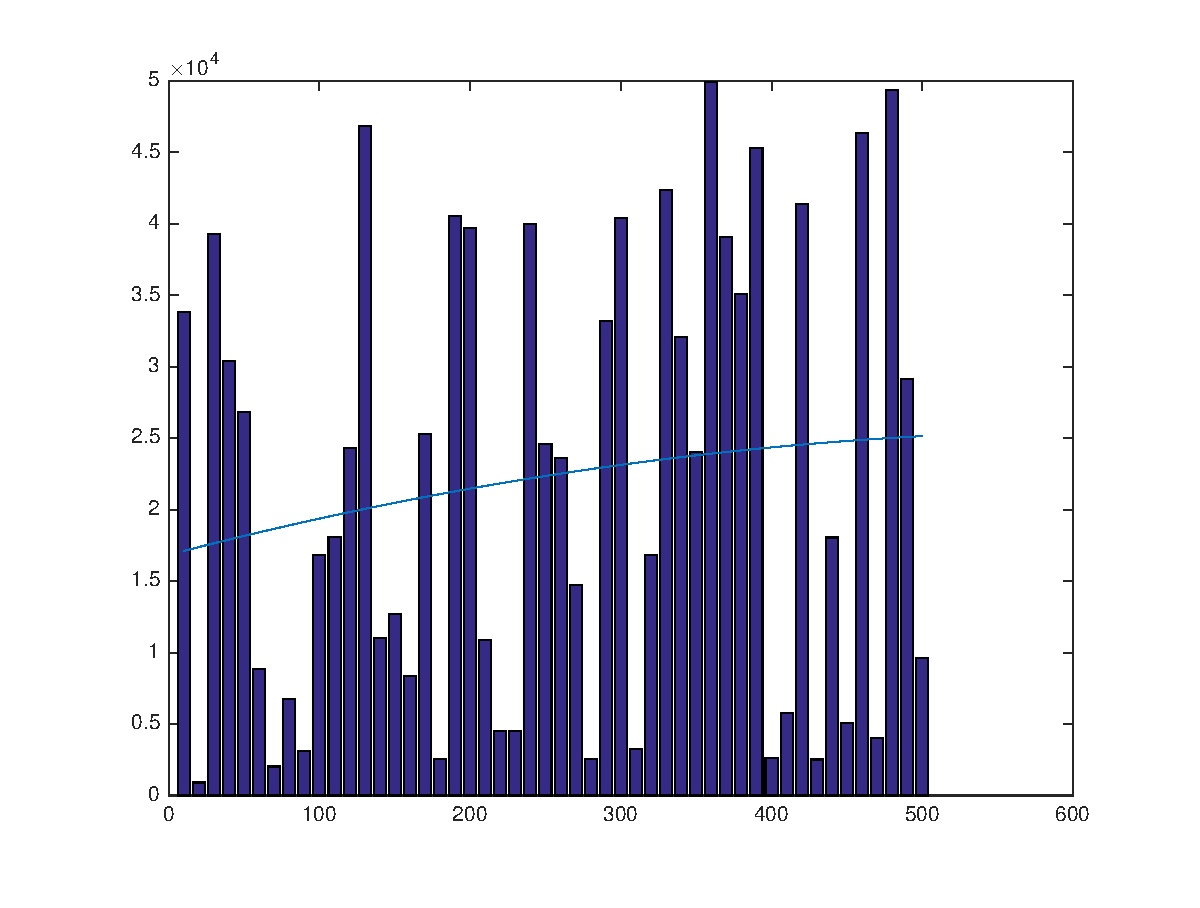
\includegraphics[width=\textwidth]{tamPob}
\caption{Gráfico de barras que representa en el eje X el tamaño de la poblacion y en el Y el número de "iteraciones útiles". Hemos añadido una aproximación de grado 2 para mostrar la tendencia.}
\label{fig:tamPob}
\end{figure}
Con poblaciones pequeñas el algoritmo parece estancarse antes.En la figura \ref{fig:tamPob} la línea clara indica la tendencia. Si la hay es muy pequeña.
\paragraph{Mutaciones}
No he encontrado una relación directa entre la \textbf{probabilidad de mutación} y la efectividad del algoritmo. Si puedo decir que \textbf{no debe ser nula} para evitar que el algoritmo se estanque. También puedo decir que está relacionada con el tamaño de la población, ya que o bien generas muchos individuos en el origen (con una población mayor) o bien haces que los existentes muten (con este parámetro). \par
Respecto al \textbf{método de mutación}, Parece que la mutacion por inversión funciona mejor. Veanse las figuras \ref{fig:mut1} y \ref{fig:mut2}. Con mutación por inversión el algoritmo parece converger ligeramente más lento pero encuentra una solución mejor siempre prácticamente.
\begin{Verbatim}
Sin mutacion:
N= 29   20000i (    6501) P200 pM3 0.00  Ruleta ER :: fit 0.99 BD 2042/2020 :: t:12.273s
N= 29   20000i (    6965) P200 pM3 0.00  Ruleta OX :: fit 0.85 BD 2376/2020 :: t:2.112s
N= 29   20000i (     121) P200 pM3 0.00  Torneo OX :: fit 0.53 BD 3829/2020 :: t:2.159s
N= 29   20000i (     124) P200 pM3 0.00  Torneo ER :: fit 0.55 BD 3643/2020 :: t:9.927s
N= 29   20000i (     238) P200 pM3 0.00  Torneo ER :: fit 0.61 BD 3298/2020 :: t:9.761s
N= 29   20000i (    7712) P200 pM3 0.00  Ruleta OX :: fit 0.92 BD 2198/2020 :: t:2.089s
N= 29   20000i (     127) P200 pM3 0.00  Torneo ER :: fit 0.64 BD 3175/2020 :: t:9.749s
N= 29   20000i (     194) P200 pM3 0.00  Torneo OX :: fit 0.59 BD 3450/2020 :: t:2.101s
N= 29   20000i (   13656) P200 pM3 0.00  Ruleta ER :: fit 0.99 BD 2033/2020 :: t:12.342s
N= 29   20000i (     169) P200 pM3 0.00  Torneo ER :: fit 0.64 BD 3157/2020 :: t:9.937s
N= 29   20000i (     337) P 50 pM3 0.00  Ruleta OX :: fit 0.60 BD 3383/2020 :: t:2.421s
N= 29   20000i (    1208) P 50 pM3 0.00  Ruleta OX :: fit 0.76 BD 2674/2020 :: t:2.538s
N= 29   20000i (    1338) P 50 pM3 0.00  Ruleta ER :: fit 0.77 BD 2612/2020 :: t:12.107s
N= 29   20000i (     888) P 50 pM3 0.00  Ruleta OX :: fit 0.69 BD 2922/2020 :: t:2.454s
N= 29   20000i (       6) P 50 pM3 0.00  Torneo ER :: fit 0.45 BD 4485/2020 :: t:11.626s
Con mutacion por inversion, probabilidad aleatoria
N= 29   20000i () P 50 pM3 0.00  Torneo OX :: fit 0.40 BD 5065/2020 :: t:2.470s
N= 29   20000i (     390) P 50 pM3 0.00  Ruleta OX :: fit 0.58 BD 3466/2020 :: t:2.377s
N= 29   20000i (    1585) P 50 pM3 0.00  Ruleta ER :: fit 0.83 BD 2420/2020 :: t:11.975s
N= 29   20000i (     719) P 50 pM3 0.00  Ruleta OX :: fit 0.64 BD 3180/2020 :: t:2.496s
N= 29   20000i () P 50 pM3 0.00  Torneo OX :: fit 0.40 BD 5086/2020 :: t:2.570s
N= 29   20000i (   16729) P 50 pM3 0.85  Torneo ER :: fit 0.94 BD 2152/2020 :: t:9.810s
N= 29   20000i (   13148) P 50 pM3 0.88  Torneo ER :: fit 0.96 BD 2099/2020 :: t:12.598s
N= 29   20000i (   19927) P 50 pM3 0.95  Ruleta ER :: fit 0.97 BD 2076/2020 :: t:17.730s
N= 29   20000i (   10204) P 50 pM3 0.10  Torneo OX :: fit 0.96 BD 2107/2020 :: t:2.544s
N= 29   20000i (     791) P 50 pM3 0.84  Torneo OX :: fit 0.97 BD 2074/2020 :: t:2.876s
N= 29   20000i (   14400) P 50 pM3 0.02  Ruleta OX :: fit 0.91 BD 2232/2020 :: t:2.412s
N= 29   20000i (    4804) P 50 pM3 0.36  Ruleta OX :: fit 0.95 BD 2129/2020 :: t:2.646s
N= 29   20000i (    5838) P 50 pM3 0.46  Ruleta OX :: fit 0.98 BD 2071/2020 :: t:2.703s
N= 29   20000i (    9376) P 50 pM3 0.82  Torneo ER :: fit 0.90 BD 2247/2020 :: t:12.827s
N= 29   20000i (    7351) P 50 pM3 0.10  Torneo OX :: fit 0.93 BD 2179/2020 :: t:2.622s
\end{Verbatim}
\begin{figure}
	\begin{subfigure}[H]{0.50\textwidth}
		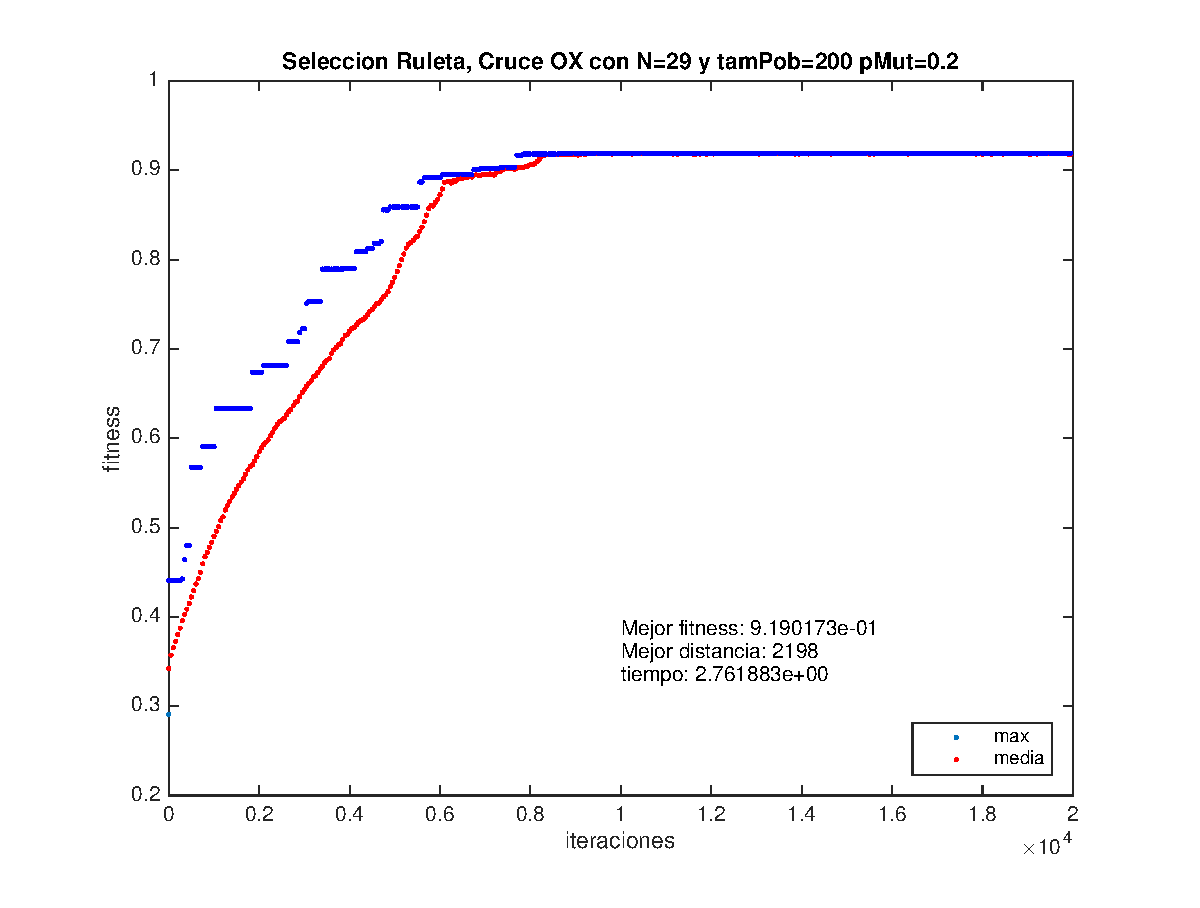
\includegraphics[width=\linewidth]{mut1b}
	\end{subfigure}
	\begin{subfigure}[H]{0.50\textwidth}
		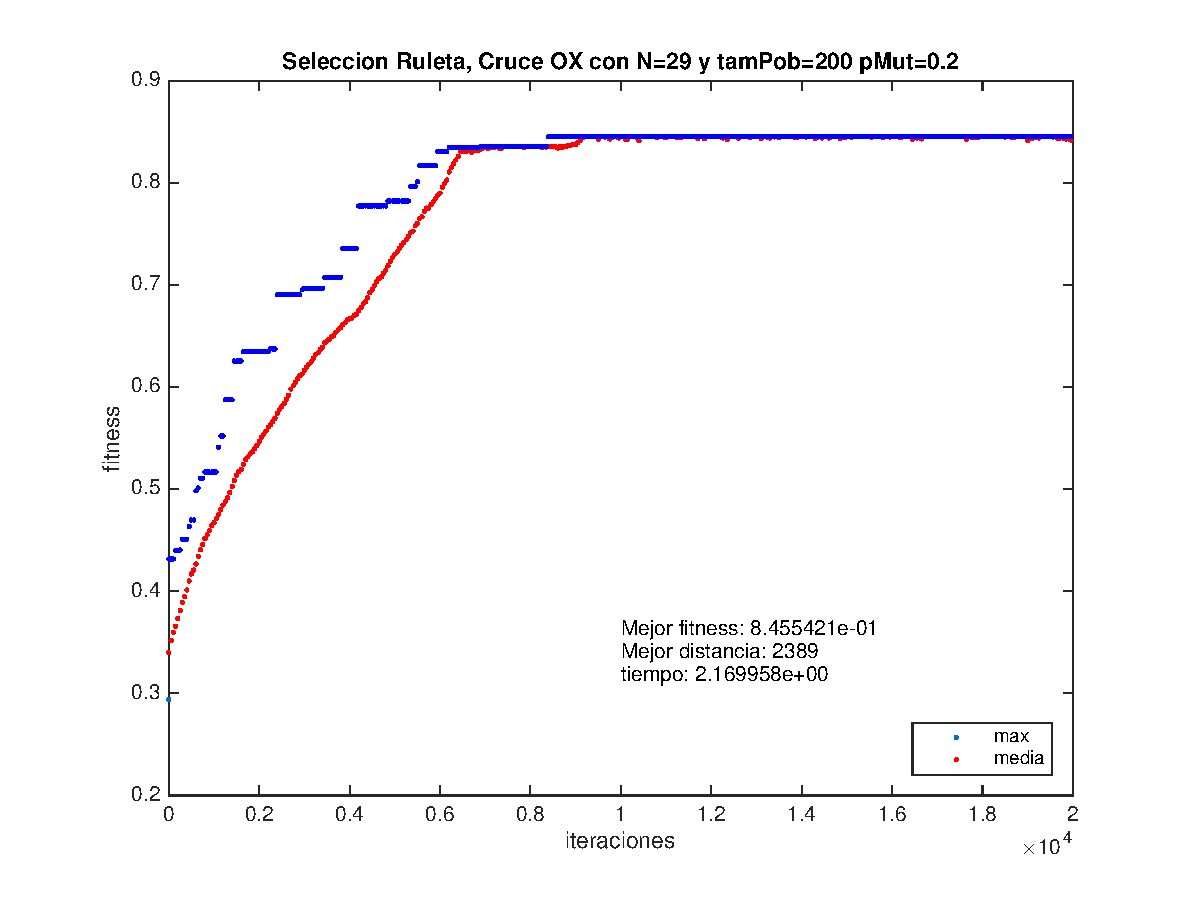
\includegraphics[width=\linewidth]{mut2b}
	\end{subfigure}
	\caption{Mutacion por insercion y por sacudida}
	\label{fig:mut1}
\end{figure}
\begin{figure}
	\begin{subfigure}[H]{0.50\textwidth}
		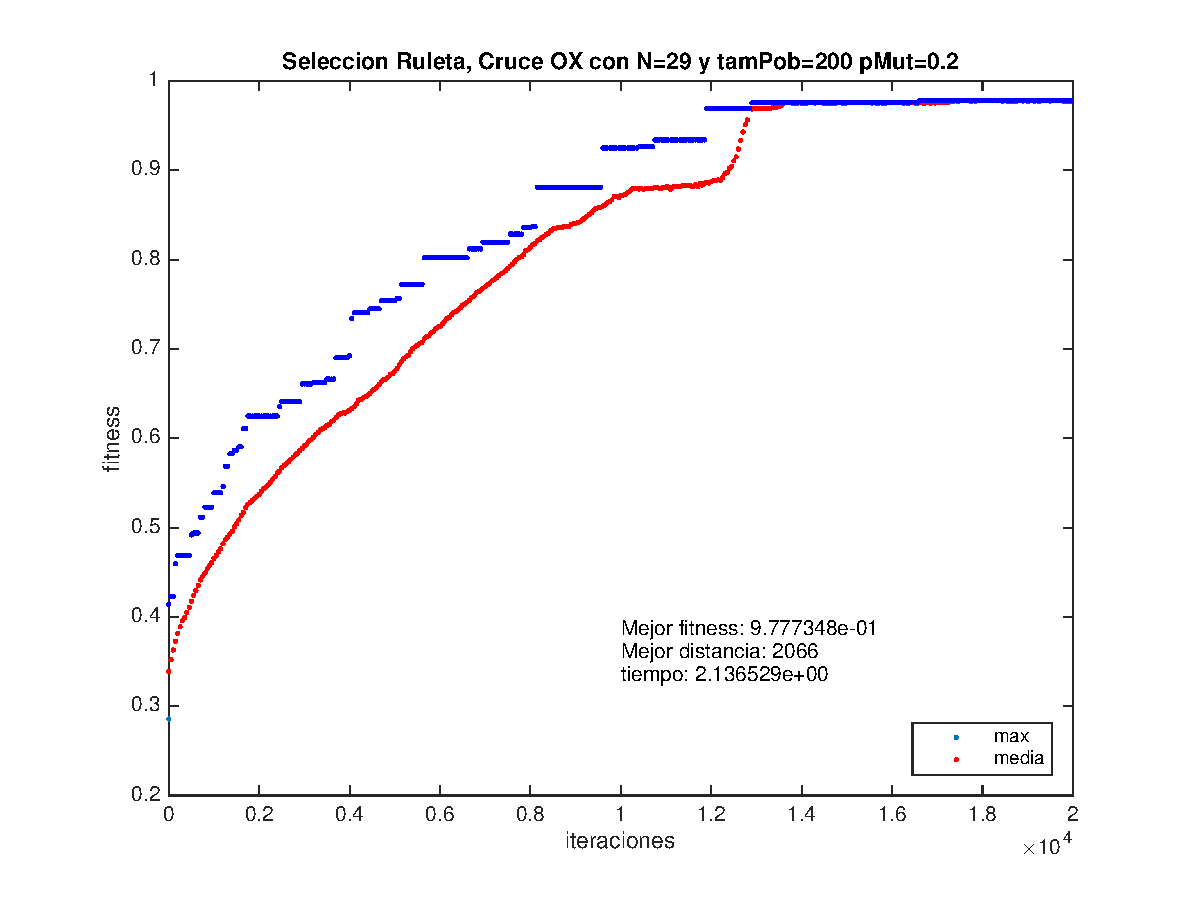
\includegraphics[width=\linewidth]{mut3b}
	\end{subfigure}
	\begin{subfigure}[H]{0.50\textwidth}
		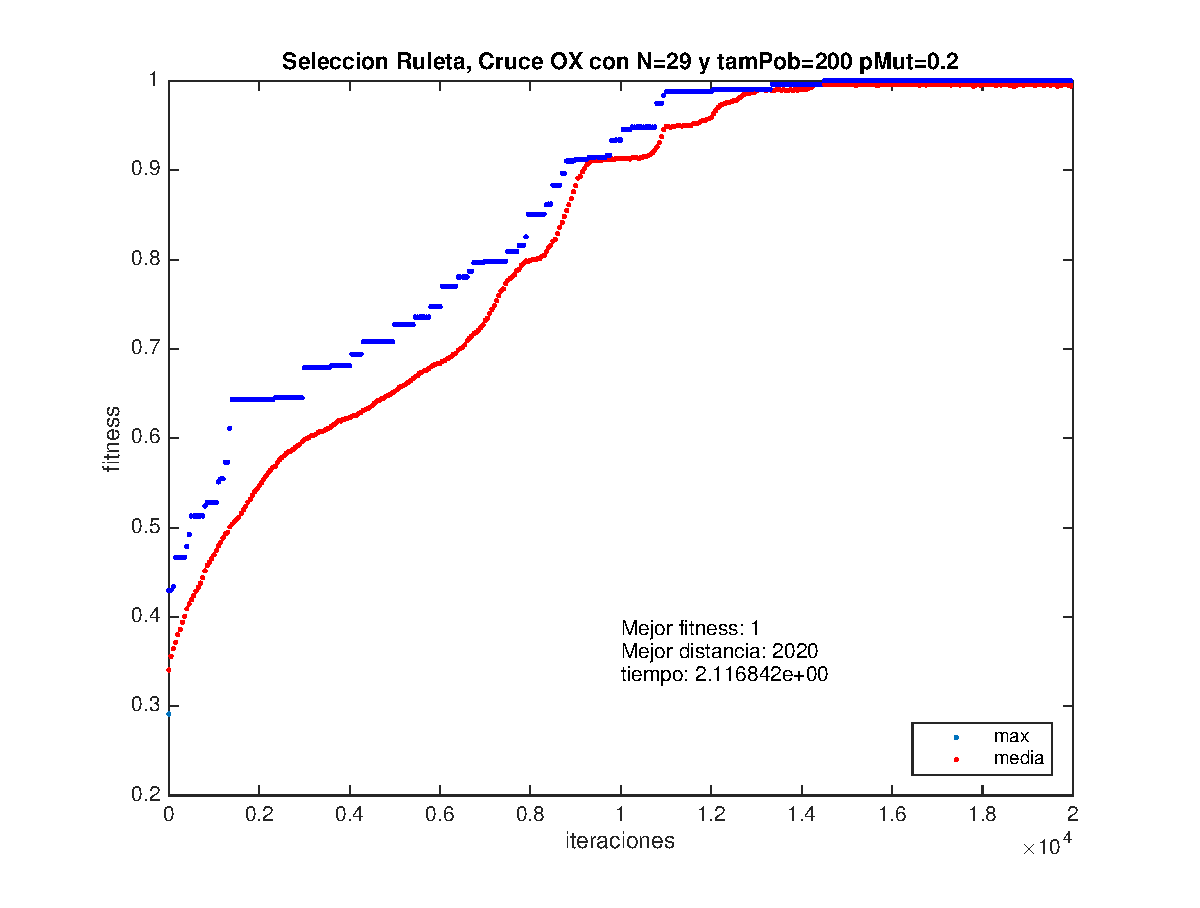
\includegraphics[width=\linewidth]{mut4b}
	\end{subfigure}
	\caption{Mutacion por inversión}
	\label{fig:mut2}
\end{figure}

\paragraph{Cruzamiento}
El cruzamiento OX es mucho más rápido y converge deprisa, pero a veces encuentra soluciones malas. En cambio el cruzamiento ER parece más fiable, pero el tiempo de ejecución es varias veces mayor. Prefiero usar el OX con un tamaño de población grande o repitiendo la ejecución varias veces para tomar la mejor solución. Pueden verse los datos anteriores con cruzamiento aleatorio. O los gráficos que ya pusimos.
\paragraph{Seleccion}
La selección por torneo permite una convergencia mucho más rápida que la selección por ruleta. Computacionalmente son parecidos. No puedo afirmar que uno sea mejor que el otro ya que dependerá de otros parámetros como la probabilidad de mutación. Si buscas una selección elitista usa el torneo. Cuanto mayor K se use en el torneo, más elitista será el genético. \\
Entre los dos métodos me gusta más el de torneo ya que podemos ajustar con el parámetro K el nivel de "elitismo".\\
Al seleccionar los cromosomas que se van fuera siempre hemos tomado a los menos aptos de la población, no hemos barajado otros métodos.
\section{Comentarios sobre el trabajo}
El documento lo he realizado con \LaTeX, el código fuente está disponible en github(\href{https://github.com/Ameb/LaTeX-Projects}{link}). Los gráficos se han realizado con MATLAB y exporando a postscript. El código lo he optimizado en la medida de lo posible, utilizando uint16 para que sobretodo el cálculo por fuerza bruta no consuma toda la memoria del sistema (puede que de error en ordenadores con pocos recursos). Se ha definido una función setdiff que funciona bien para vectores de enteros y es 10 veces más rápida que la de la libreria de matlab.
\begin{thebibliography}{1}
 	\bibitem{jess} Jessica A. Carballido, Ignacio Ponzoni, Nélida B. Brignole {\em 
	TÉCNICAS EVOLUTIVAS PARA EL PROBLEMA DEL VIAJANTE} Bahía Blanca, Argentina, Noviembre 2003.
 	
 	\bibitem{larra}  P.Larrañaga et al {\em Genetic Algorithms for the Travelling Salesman Problem: A review of Representations and Operators} Universidad del Pais Vasco, E-20080 Donostia - San Sebastián, 1999
 	
 	\bibitem{TSPLib} TSPlib: \url{http://elib.zib.de/pub/mp-testdata/tsp/tsplib/tsp/} Datasets de problemas TSP con sus soluciones.
\end{thebibliography}
\end{document}
